\section{Benchmark Design}

\subsection{Generation Pipeline}

The generator maintains a ledger whose sign convention follows normal accounting balances: assets and expenses increase on debits, while liabilities, equity, and revenue increase on credits.
Every transaction is applied to this ledger, and the final balance sheet is derived directly from the resulting account state.
Revenue and expense balances are folded into Retained Earnings when the final balance sheet is built, making closing-entry competence observable in the model outputs.

Transaction templates are organized by difficulty level and accounting feature.
Lower levels emphasize basic cash bookkeeping; higher levels activate credit transactions, debt servicing, prepaids, depreciation, cost-of-goods-sold coupling, derived-interest calculations, and mixed-funding purchases.
Adjustments are generated separately and applied before the statement is prepared.
The full benchmark is deterministic given a random seed, and the released corpus contains 2{,}500 problems.

\begin{table*}[t]
\centering
\small
\resizebox{\textwidth}{!}{%
\begin{tabular}{lrrrrl}
\toprule
Level & Problems & Avg.\ tx/problem & Avg.\ accounts & Avg.\ adjustments & Characteristic factors \\
\midrule
L1 & 500 & 7.56 & 5.18 & 0.00 & cash-only core with prepaids and basic depreciable assets \\
L2 & 750 & 14.79 & 8.38 & 0.72 & credit transactions, debt, and expiring prepaids \\
L3 & 750 & 27.39 & 11.61 & 1.68 & COGS-linked sales, accruals, depreciation, derived interest \\
L4 & 400 & 47.55 & 14.16 & 3.16 & mixed-funding purchases and dense adjustment chains \\
L5 & 100 & 79.35 & 15.22 & 4.57 & all complexity factors active in the same problem \\
\bottomrule
\end{tabular}
}
\caption{Dataset composition. Difficulty scales both the number of journal events and the number of simultaneously active accounting mechanisms.}
\label{tab:dataset-summary}
\end{table*}


Table~\ref{tab:dataset-summary} shows that difficulty is not cosmetic.
Average transactions increase from $7.56$ at Level~1 to $79.35$ at Level~5, while average account support rises from $5.18$ to $15.22$.
The generator therefore scales both event count and latent bookkeeping structure.

\begin{figure*}[t]
\centering
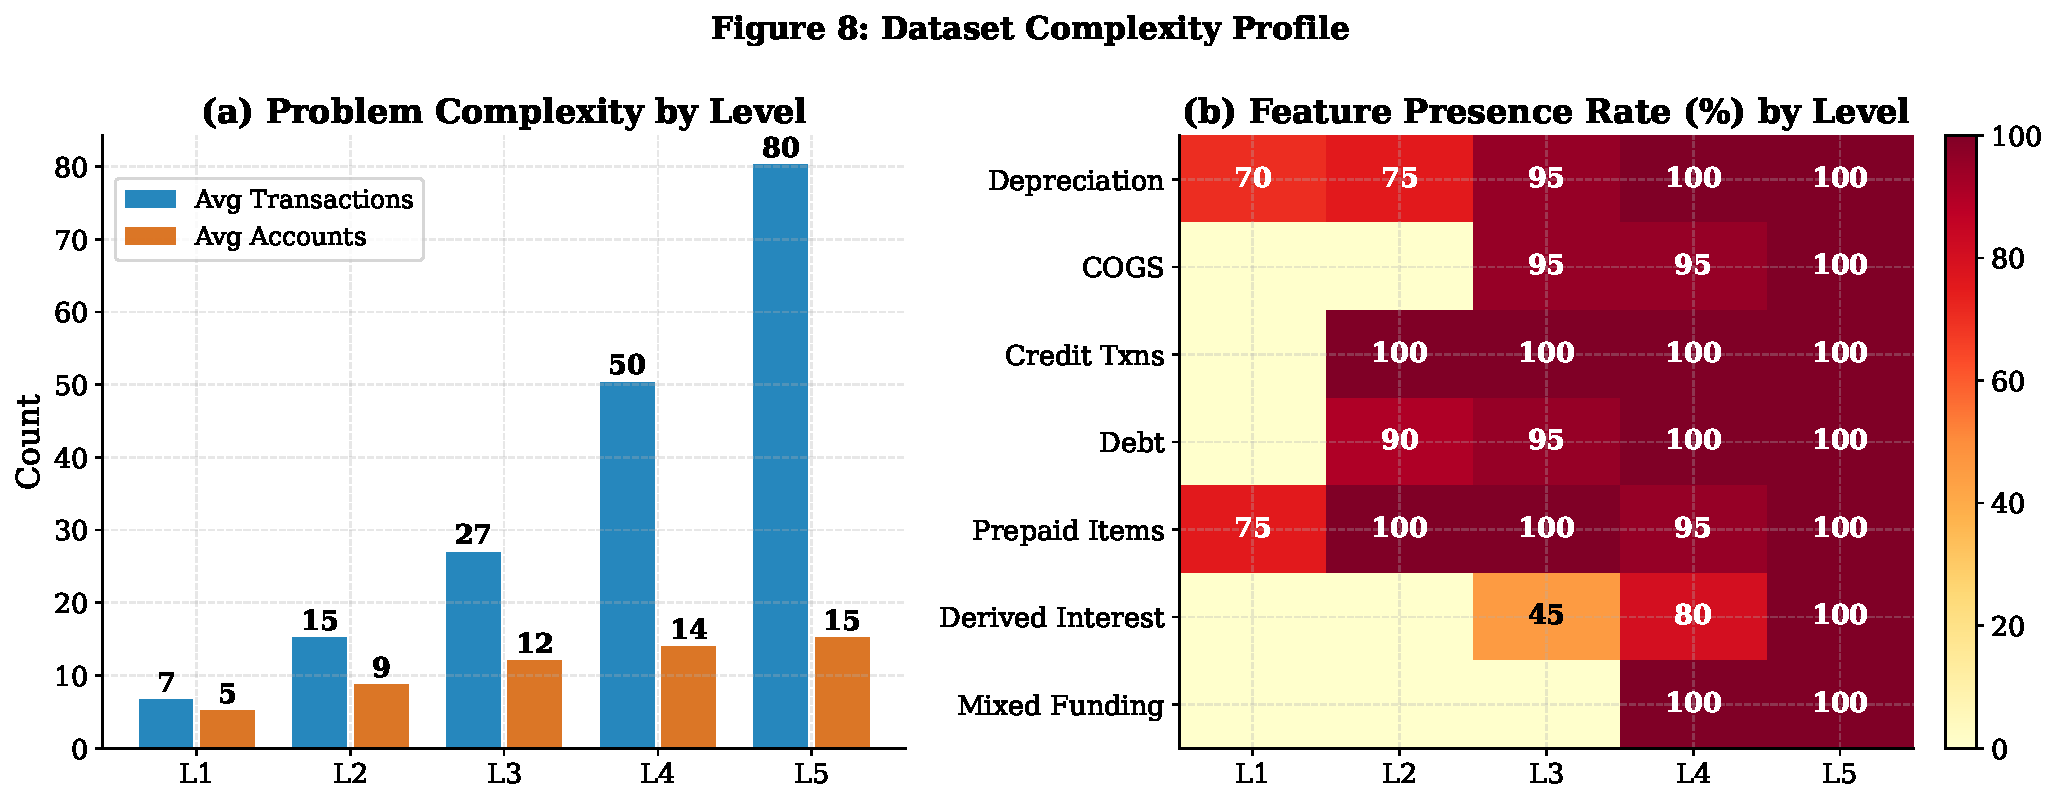
\includegraphics[width=0.95\textwidth]{../figures/F8_dataset_complexity.pdf}
\caption{Dataset complexity profile. Panel (a) shows the mean number of transactions and distinct non-zero balance-sheet accounts per problem at each difficulty level. Panel (b) shows the percentage of problems at each level containing each accounting mechanism. Higher levels therefore increase both bookkeeping volume and mechanism diversity.}
\label{fig:dataset-complexity}
\end{figure*}

Figure~\ref{fig:dataset-complexity} should be read panel by panel.
In panel~(a), the x-axis is difficulty level (L1--L5) and the y-axis
is a count; the blue bars show the mean number of journal
transactions, while the orange bars show the mean number of distinct
accounts in the expected final statement.
The point is that harder levels are not just longer prompts:
they require the model to maintain more latent account states as well.
Panel~(b) uses the same x-axis but changes the y-axis to feature type
and the color scale to the percentage of problems at that level that
contain the feature.
\emph{Depreciation} means depreciable fixed assets together with their
end-of-period depreciation adjustment;
\emph{COGS} means sales paired with inventory relief and
cost-of-goods-sold recognition;
\emph{Credit Txns} means receivable/payable transactions rather than
pure cash flows;
\emph{Debt} means loans, notes, or their repayment/accrual;
\emph{Prepaid Items} means prepaid rent or insurance later expired into
expense;
\emph{Derived Interest} means interest computed from principal, rate,
and time rather than copied directly from a stated amount; and
\emph{Mixed Funding} means fixed-asset purchases split between cash and
debt.
The main takeaway is that Levels~4--5 add interacting accounting
mechanisms, not just more rows.
Difficulty is staged progressively across all five levels.
Level~1 contains 5--10 mostly cash transactions and no end-of-period
adjustments, so the task is basic ledger accumulation.
Level~2 introduces credit sales and purchases, receivables/payables,
debt, and a single adjustment.
Level~3 expands to 20--35 transactions plus 1--3 adjustments such as
depreciation, accruals, bad-debt provision, and COGS-coupled sales.
Level~4 adds mixed-funded fixed-asset purchases and chained
adjustments, so multiple mechanisms must be coordinated in one
statement.
Level~5 uses the same mechanism set at the highest density, typically
60--100 transactions with 3--5 adjustments, making long-horizon
bookkeeping and closing especially difficult.
Appendix~\ref{app:difficulty-samples} gives abbreviated sample problems
for Levels~1--5.

\subsection{Prompted Task}

\benchmark{} evaluates whether a model can prepare a valid balance sheet from the provided ledger state and transaction stream.
\zs{} asks for a JSON answer directly with a reminder that Assets must equal Liabilities plus Equity.
Reflective \CoT{} asks the model to reason step by step and then emit a final JSON object after the marker \texttt{FINAL ANSWER:}.
These are the two evaluated prompting conditions in this paper.

\begin{center}
\fbox{%
\begin{minipage}{0.95\columnwidth}
\textbf{Sample benchmark entry.}

\vspace{4pt}
\footnotesize
\texttt{Opening balances: Cash 49,400; Owner's Equity 49,400}

\texttt{Transactions:}

\texttt{1. Dr Equipment 17,700 / Cr Cash 17,700}

\texttt{2. Dr Operating Expenses 200 / Cr Cash 200}

\texttt{3. Dr Prepaid Rent 5,900 / Cr Cash 5,900}

\texttt{4. Dr Prepaid Rent 3,400 / Cr Cash 3,400}

\texttt{5. Dr Cash 20,600 / Cr Owner's Equity 20,600}

\vspace{4pt}
\texttt{Expected JSON output:}

\texttt{\{"assets": \{"Cash": 42800, "Equipment": 17700, "Prepaid Rent": 9300\},}

\texttt{"liabilities": \{\},}

\texttt{"equity": \{"Owner's Equity": 70000, "Retained Earnings": -200\}\}}
\end{minipage}}
\end{center}

Appendix~\ref{app:worked-example} provides a full worked pipeline
example for this task, including the prompted input, intermediate
ledger updates, the retained-earnings closure step, and the final
expected JSON output.
Appendix~\ref{app:difficulty-samples} additionally provides abbreviated
sample problems for each of the five difficulty levels.

\subsection{Metrics and Error Taxonomy}

No single score captures this task well because models can produce
the right account set while still failing the bookkeeping.
\ba{} (balance accuracy) is therefore a hard binary check:
it equals \(1\) only when the predicted statement satisfies
\(|A-(L+E)| \leq 1\) currency unit.
\ala{} (account-level accuracy) measures the fraction of expected
non-zero accounts whose predicted values fall within a hybrid
tolerance of \(\max(\$10, 1\%\ \text{of expected value})\); omitted
accounts count as incorrect.
\acr{} (account coverage rate) ignores values and asks only whether
the expected accounts appear anywhere in the output, which isolates
structural recall from numerical correctness.
\cecr{} (closing-entry compliance rate) checks whether Retained
Earnings is present in equity and numerically correct under the same
hybrid tolerance; if Retained Earnings is not expected, the instance
is treated as trivially compliant.

We report four secondary diagnostics to make failure modes more
interpretable.
\textsc{BEM} (balance error magnitude) is the continuous version of
\ba{}, defined as \(|A-(L+E)|\).
Section placement accuracy (SPA) is the fraction of predicted
accounts assigned to the correct top-level section
(\texttt{assets}, \texttt{liabilities}, or \texttt{equity}).
Hallucination rate (HR) is the fraction of predicted accounts that
do not belong in the expected final statement.
Constraint satisfaction rate (CSR) is the proportion of benchmark
constraints satisfied, including the balance equation, non-negative
non-contra assets, contra-asset sanity, non-negative total assets,
and completeness of the expected account set.
Numerical error is summarized with MAE and RMSE over expected
accounts, treating missing values as zero.

The main scalar summary is \fbs{}, a \(0\)--\(100\) weighted
aggregate of \ba{}, \ala{}, CSR, and normalized numerical error
\(1-\min(\text{MAE}/50{,}000, 1)\).
For the no-intermediate-state setting used in this paper, the
weights are \(0.375\) for \ba{}, \(0.3125\) for \ala{},
\(0.1875\) for CSR, and \(0.125\) for normalized numerical error.
If intermediate ledger states are available, the transaction
processing accuracy term receives weight \(0.20\), and the remaining
weights revert to \(0.30\), \(0.25\), \(0.15\), and \(0.10\),
respectively.

The error taxonomy complements these metrics.
We distinguish arithmetic errors (wrong values on present accounts,
for example Cash reported as \(12{,}400\) instead of \(13{,}400\)),
omission errors (missing expected accounts, such as an omitted
Accumulated Depreciation line), hallucinations (extra unsupported
accounts, such as Goodwill), classification errors (correct accounts in
the wrong section, such as Notes Payable under equity), constraint
violations (global bookkeeping breaks such as
\(A \neq L + E\) or a positive Accumulated Depreciation balance), and
formatting/parsing failures (malformed or non-JSON outputs that cannot
be scored reliably).
When intermediate states are available, repeated downstream mistakes
are additionally marked as propagation errors, for example an early
Accounts Receivable mistake that later distorts both cash collections
and ending equity.
Secondary analyses aggregate these per-problem signals into
complexity-factor reports, account-difficulty indices, difficulty
curves, and permutation-test summaries.
